\section{Codeforces Beta Round \#2 -- Problem C: Commentator Problem}

\begin{frame}[fragile]{Problema}

The Olympic Games in Bercouver are in full swing now. Here everyone has their own objectives: sportsmen compete for medals, and sport commentators compete for more convenient positions to give a running commentary. Today the main sport events take place at three round stadiums, and the commentator's objective is to choose the best point of observation, that is to say the point from where all the three stadiums can be observed. As all the sport competitions are of the same importance, the stadiums should be observed at the same angle. If the number of points meeting the conditions is more than one, the point with the maximum angle of observation is prefered.

Would you, please, help the famous Berland commentator G. Berniev to find the best point of observation. It should be noted, that the stadiums do not hide each other, the commentator can easily see one stadium through the other.

\end{frame}

\begin{frame}[fragile]{Entrada e saída}

\textbf{Input}

The input data consists of three lines, each of them describes the position of one stadium. The lines have the format $x, y, r$, where $(x, y)$ are the coordinates of the stadium's center 
$(-10^3\leq x, y\leq 10^3)$, and $r$ $(1\leq r\leq 10^3)$ is its radius. All the numbers in the input data are integer, stadiums do not have common points, and their centers are not on the same line.

\textbf{Output}

Print the coordinates of the required point with five digits after the decimal point. If there is no answer meeting the conditions, the program shouldn't print anything. The output data should be left blank.

\end{frame}

\begin{frame}[fragile]{Exemplo de entradas e saídas}

\begin{minipage}[t]{0.5\textwidth}
\textbf{Sample Input}
\begin{verbatim}
0 0 10
60 0 10
30 30 10
\end{verbatim}
\end{minipage}
\begin{minipage}[t]{0.45\textwidth}
\textbf{Sample Output}
\begin{verbatim}
30.00000 0.00000
\end{verbatim}
\end{minipage}
\end{frame}

\begin{frame}[fragile]{Solução}

    \begin{itemize}
        \item Uma estratégia útil para solucionar um problema sofisticado é trabalhar com
            casos mais simples, que permitam a identificação de relações e propriedades
            das variáveis do problema

        \item Considere o caso de apenas dois estádios circulares com centros $P$ e $Q$, e
        que ambos tenham o mesmo raio $r$
    \end{itemize}

    \begin{figure}
        \centering

        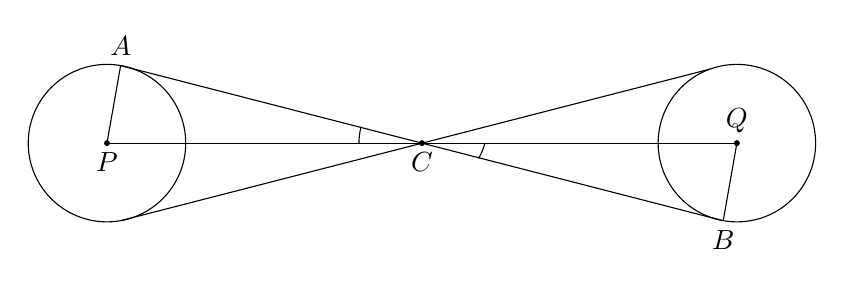
\begin{tikzpicture}
            \draw (0, 0) circle (1);
            \draw[fill] (0, 0) circle (0.03);
            \draw (8, 0) circle (1);
            \draw[fill] (8, 0) circle (0.03);
            \draw[fill] (4, 0) circle (0.03);

            \draw (0, 0) -- (8, 0);
            \draw ({ cos(280) }, { sin(280) }) -- ({ cos(110) + 8 }, { sin(110) });
            \draw ({ cos(80) }, { sin(80) }) -- ({ cos(260) + 8 }, { sin(260) });
            \draw (0, 0) -- ({ cos(80) }, { sin(80) });
            \draw (8, 0) -- ({ cos(260) + 8 }, { sin(260) });

            \node[anchor=north] at (0, 0) { $P$ };
            \node[anchor=south] at (8, 0) { $Q$ };
            \node[anchor=north] at (4, 0) { $C$ };
            \node[anchor=south] at ( { cos(80) }, { sin(80) } ) { $A$ };
            \node[anchor=north] at ( { 8 + cos(260) }, { sin(260) } ) { $B$ };

            \draw (3.2, 0) arc [radius=0.8, start angle=180, delta angle=-15];
            \draw (4.8, 0) arc [radius=0.8, start angle=345, delta angle=-15];
        \end{tikzpicture}
    \end{figure}
\end{frame}

\begin{frame}[fragile]{Solução}

    \begin{itemize}
        \item Os segmentos $AP$ e $BQ$ tem comprimento $r$

        \item Os triângulos $PAC$ e $QBC$ são retângulos e congruentes

        \item Logo, a distância do ponto ideal $C$ aos centros $P$ e $Q$ deve ser a mesma

        \item O conjunto de pontos que satisfaz a condição $d(P, C) = d(Q, C)$ é a mediatriz do
            segmento $PQ$

        \item O parâmetros da mediatriz são dados por
        \begin{align*}
            0 &= d^2(P, C) - d^2(Q, C) \\
            &= (x - x_P)^2 + (y - y_P)^2 - (x - x_Q)^2 - (y - y_Q)^2 \\
            &= -2(x_P - x_Q)x -2(y_P - y_Q)y + (x_P^2 + y_P^2 - x_Q^2 - y_Q^2)
        \end{align*}
            
        \item Se os raios dos três estádios são idênticos, a solução será a interseção de 
            duas das mediatrizes, se existir
    \end{itemize}

\end{frame}

\begin{frame}[fragile]{Solução}

    \begin{itemize}
        \item Considere agora o caso onde os raios $r_P$ e $r_Q$ são distintos
    \end{itemize}

    \begin{figure}
        \centering

        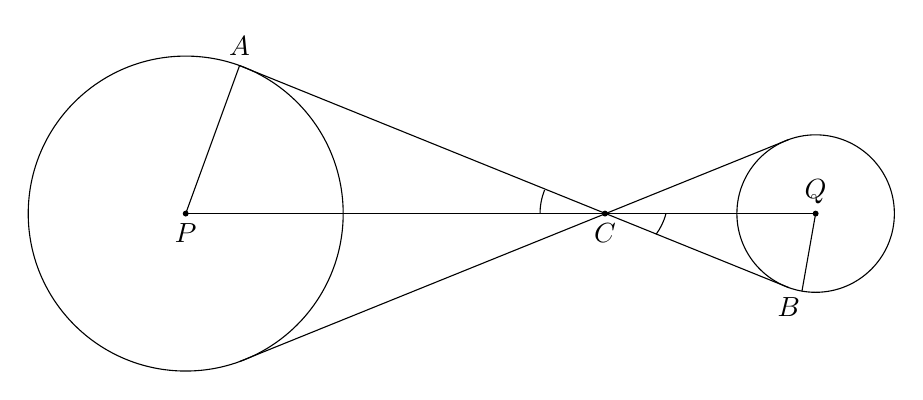
\begin{tikzpicture}
            \draw (0, 0) circle (2);
            \draw[fill] (0, 0) circle (0.03);
            \draw (8, 0) circle (1);
            \draw[fill] (8, 0) circle (0.03);
            \draw[fill] (5.325, 0) circle (0.03);

            \draw (0, 0) -- (8, 0);
            \draw ({ 2*cos(290) }, { 2*sin(290) }) -- ({ cos(110) + 8 }, { sin(110) });
            \draw ({ 2*cos(70) }, { 2*sin(70) }) -- ({ cos(250) + 8 }, { sin(250) });
            \draw (0, 0) -- ({ 2*cos(70) }, { 2*sin(70) });
            \draw (8, 0) -- ({ cos(260) + 8 }, { sin(260) });

            \node[anchor=north] at (0, 0) { $P$ };
            \node[anchor=south] at (8, 0) { $Q$ };
            \node[anchor=north] at (5.325, 0) { $C$ };

            \node[anchor=south] at ( { 2*cos(70) }, { 2*sin(70) } ) { $A$ };
            \node[anchor=north] at ( { 8 + cos(250) }, { sin(250) } ) { $B$ };

            \draw (4.5, 0) arc [radius=0.8, start angle=180, delta angle=-22];
            \draw (6.1, 0) arc [radius=0.8, start angle=345, delta angle=-21];
        \end{tikzpicture}
    \end{figure}

\end{frame}

\begin{frame}[fragile]{Solução}

    \begin{itemize}
        \item Neste caso, os triângulos $PAC$ e $QBC$ são semelhantes, mas não congruentes

        \item Da congruência segue que
        \[
            \frac{d(P, C)}{r_P} = \frac{d(Q, C)}{r_Q}
        \] 

        \item Daí
        \begin{align*}
        0 &= r_Q^2d^2(P, C) - r_P^2d^2(Q, C) \\
        &= r_Q^2\left[(x - x_P)^2 + (y - y_P)^2\right] - r_P^2\left[(x - x_Q)^2 + (y -y_Q)^2\right]\\
        &= \left[ (r_Q^2 - r_P^2)x^2 -2x(r_Q^2x_P - r_P^2x_Q) \right] \\
        &+ \left[ (r_Q^2 - r_P^2)y^2 -2y(r_Q^2y_P - r_P^2y_Q) \right] + \left[ x_P^2 + y_P^2 - x_Q^2 - y_Q^2\right]
        \end{align*}
    \end{itemize}

\end{frame}

\begin{frame}[fragile]{Solução}

    \begin{itemize}
        \item Seja
        \[
            x_0 = \frac{r_Q^2x_P - r_P^2x_Q}{r_Q^2 - r_P^2}\ \ \ \mbox{e}\ \ \ 
            y_0 = \frac{r_Q^2y_P - r_P^2y_Q}{r_Q^2 - r_P^2}
        \]

        \item Completando o quadrado em $x$ e em $y$ segue que
        \[
            (x - x_0)^2 + (y - y_0)^2 = R^2,
        \]
        onde
        \[
            R = \frac{r_Q^2(x_P^2 + y_P^2) - r_P^2(x_Q^2 - y_Q^2)}{r_Q^2 - r_P^2} - x_0^2 - y_0^2
        \]

        \item Neste caso, a solução será, dentre as duas possíveis interseções entre os 
            círculos correspondentes à dois pares de estádios com raios distintos, a que 
            produz o maior ângulo

        \item Este ângulo $\alpha$ é dado por
        \[
            \alpha = 2\arcsin\left(\frac{r_P}{d(P, C)}\right)
        \]
    \end{itemize}

\end{frame}
\begin{frame}[fragile]{Solução AC com complexidade $O(n \log n)$}
%    \inputsnippet{cpp}{1}{21}{ac2.cpp}
\end{frame}

